\chapter{Dimensionamento Estrutural}

\section{Dimensionamento Estrutural da Asa}

\subsection{Dimensionamento das longarinas}
A partir do esforços apresentados nas figuras \ref{fig:cort_ASA}, \ref{fig:flet_ASA} e \ref{fig:torc_ASA}, pode-se realizar um dimensionamento das longarinas 1 e 2 da asa, utilizando o momento de inércia de cada seção, o momento fletor atuante e a distância do centro da seção até as extremidades, onde o valor da tensão é o máximo.

Considerou-se durante este dimensionamento que as longarinas serão fabricadas de uma liga de alumínio da série 7000, Al 7050-T7451, devido a maior facilidade de projeto, construção e manutenção. No dimensionamento o valor de tensão obtido em cada seção foi comparado ao limite de resistência do material selecionado, aplicando-se um fator de material de 1.15.
Considerou-se a existência de duas longarinas em perfil I, formando com o revestimento, um caixão principal capaz de suportar os esforços de torção na asa, e considerou-se que as longarinas suportariam sozinhas os esforços fletores.
Os resultados obtidos do dimensionamento estrutural das longarinas estão apresentados na \autoref{tbl:longarinas2} e foram considerados satisfatórios para esta etapa de projeto.


\begin{table}[H]
\centering
\begin{tabular}{ccc}
\toprule
(mm) & Raiz & Ponta \\ \midrule
Longarina 1 &  &   \\ \midrule
Espessura mesas & 12 & 8 \\
Largura mesas & 60 & 40\\
Altura alma & 447.6 & 266.6 \\
Espessura alma & 5 & 2.5 \\ \midrule
Longarina 2 &  &   \\ \midrule
Espessura mesas & 10 & 5 \\
Largura mesas & 50 & 30 \\
Altura alma & 373.0 & 225.5 \\
Espessura alma & 5 & 2.5 \\
\bottomrule
\end{tabular}
\caption{Dimensionamento Preliminar da Longarina da Asa}
\label{tbl:longarinas2}
\end{table}

\subsection{Posicionamento das longarinas}
Com base no \cite{roskam}, foram utilizadas duas longarinas principais na asa, formando portanto uma espécie de caixão, o qual suporta os esforços principais de flexão e de torsão na asa. As longarinas que compõem o caixão devem ser posicionadas de forma que tirem o máximo de vantagem estrutural da altura do perfil.

As posições das longarinas são tipicamente como segue:
\begin{itemize}
\item Longarina dianteira: 15-30\% da corda
\item Longarina traseira: 65-75\% da corda
\end{itemize}

Neste projeto considerou-se, portanto, a longarina dianteira a 25\% da corda e a longarina traseira a 75\% da corda.

\subsection{Dimensionamento das nervuras}
Devido a razões aerodinâmicas o contorno da asa na direção da corda deve ser mantido sem distorção considerável. Portanto, são utilizadas nervuras para suportar e dar forma ao revestimento e também para limitar o tamanho dos reforçadores entre elas, gerando uma resistência de compressão eficiente. As nervuras ainda tem um outro propósito estrutural que é o de atuar como um distribuidor de carregamentos.

A \autoref{fig:nervura_asa} ilustra uma nervura típica, onde também observa-se os reforçadores da asa. Observa-se também furos de alívio nesta imagem da nervura e também janelas de inspeção.

\begin{figure}
\centering
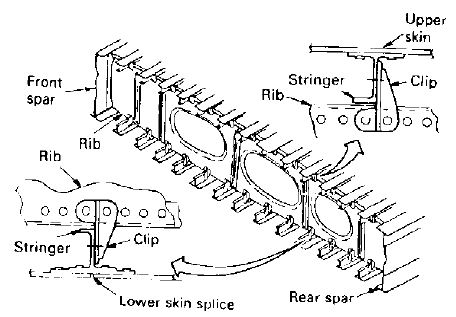
\includegraphics[width=\textwidth]{images/parte4/nervura}
\caption{Nervura típica em uma asa}
\label{fig:nervura_asa}
\end{figure}

As nervuras são dimensionadas visando cobrir as seguintes funções:
\begin{itemize}
  \item Carregamentos primários: os carregamentos primários atuantes em uma nervura são as cargas externas que devem ser transferidas para o restante da estrutura;
  \item Cargas de inércia: combustível, estrutura, equipamentos;
  \item Cargas devido aos momentos de flexão: quando a asa é submetida aos carregamentos de flexão, as nervuras são submetidas a compressão, conforme mostrado na \autoref{fig:nervura_asa2}
  \item Redistribuição de cargas concentradas: como cargas da nacele e do trem de pouso para as longarinas da asa e para os paineis de revestimento
\end{itemize}

\begin{figure}
\centering
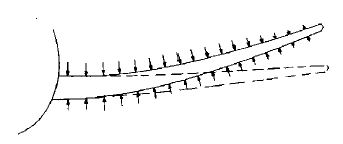
\includegraphics[width=\textwidth]{images/parte4/nervura2}
\caption{Comportamento da asa devido à flexão}
\label{fig:nervura_asa2}
\end{figure}

A análise estrutural de uma nervura consiste em analisar os seguintes itens:
\begin{itemize}
  \item Cisalhamento na alma das nervuras
  \item Cisalhamento entre as nervuras e o revestimento
  \item Cisalhamento entre as nervuras e a longarina
  \item Espaçamento entre nervuras
\end{itemize}

As nervuras, portanto, foram dimensionadas majoritariamente visando suportar o fluxo de cisalhamento que passa por elas. 
Para um dimensionamento inicial, foi selecionada a nervura mais próxima à raiz da asa, visto que os esforços solicitantes são maiores naquela região.
Obteve-se deste dimensionamento que a espessura da nervura deve ser de 3mm.

\subsection{Espaçamento entre as nervuras}
Com base no \cite{niu1999airframe} o espaçamento entre as nervuras deve ser estabelecido durante fases preliminares do projeto, visto que o peso das nervuras é significante no peso total da estrutura da asa.
Um critério extremamente importante ao avaliar o espaçamento entre as nervuras é as estabilidade da estrutura do revestimento.
O revestimento do extradorso é especialmente avaliado durante este dimensionamento, visto que ele é submentido a cargas de compressão consideráveis e quando o espaçamento entre as nervuras é muito elevado tem-se a flambagem deste revestimento.

Portanto, levando-se em conta este critério e visando manter a estabilidade da estrutura, segundo \cite{roskam}, um espaçamento típico entre nervuras para aeronaves de transporte é de no máximo 600mm.

\subsection{Reforçadores na asa}
Visando ainda auxiliar na estabilidade do painel do revestimento da asa, foram projetados reforçadores para esses paineis.
Foram colocados seis reforçadores no intradorso da asa e seis reforçadores no extradorso, espaçados de 219mm na raiz, onde é a seção crítica a flambagem para a compressão do revestimento.

Calculou-se a altura dos reforçadores para a seção crítica: no extradorso próximo à raiz da asa, onde o momento de flexão e portanto a carga de compressão é máxima.
Obteve-se então uma altura de reforçador de 40mm.
Com esta altura, a inércia gerada por estes reforçadores auxilia na estabilidade do painel.

\section{Dimensionamento Estrutural da Fuselagem}

\subsection{Espessura do revestimento}
A espessura do revestimento foi dimensionada com base na pressão de pressurização que ele deve suportar.
Os demais esforços serão suportados por esse revestimento somado aos reforçadores e cavernas.

O teto de serviço da aeronave é de 25000ft,
enquanto a cabine é pressurizada a 6000ft,
conforme definido na \autoref{sec:sys_press}.
Considerando atmosfera padrão (ISA) a diferença de pressão é de 44kPa.

O material do revestimento foi escolhido como alumínio 2024-T3, devido à sua boa resistência a corrosão, a impactos e estrutural.
Por isso ele é de emprego comum na indústria aeronáutica para revestimentos.
O limite de elasticidade desse material é de 290MPa.
Considerando um fator de segurança para o material de 1,15, o limite de escoamento fica $\sigma_y = 252\text{MPa}$.

Para um vaso de pressão cilindrico, temos
\begin{align}
\sigma_\text{long} &= \frac{pr}{2t} \\
\sigma_\theta      &= \frac{pr}{t}
\end{align}

O esforço na direção $\theta$ é claramente o dimensionante, portanto, considerando um fator de projeto de 1,5:
\begin{equation}
    t = \frac{pd}{2\sigma_y} = \frac{1,5 \cdot 44\si{kPa} \cdot 2070\si{mm}}{2 \cdot 252\si{MPa}} = 0,27\si{mm}
\end{equation}

Para aumentar a resistência a impactos e a facilidade de fabricação, a espessura do revestimento foi aumentada para $2\si{mm}$.


\section{Dimensionamento Estrutural da Empenagem}

\subsection{Empenagem horizontal}
A partir do esforços apresentados nas figuras \ref{fig:cort_EH}, \ref{fig:flet_EH} e \ref{fig:torc_EH}, pode-se realizar um dimensionamento das longarinas 1 e 2 da empenagem horizontal, utilizando o momento de inércia de cada seção, o momento fletor atuante e a distância do centro da seção até as extremidades, onde o valor da tensão é o máximo.

Assim como na estrutura da asa, considerou-se durante este dimensionamento que as longarinas serão fabricadas de uma liga de alumínio da série 7000, Al 7050-T7451, devido a maior facilidade de projeto, construção e manutenção.
No dimensionamento, o valor de tensão obtido em cada seção foi comparado ao limite de resistência do material selecionado, aplicando-se um fator de material de 1.15.
Considerou-se a existência de duas longarinas em perfil I, formando com o revestimento um caixão principal capaz de suportar os esforços de torção na empenagem.
Os resultados obtidos do dimensionamento estrutural das longarinas estão apresentados na \autoref{tbl:longarinasEH} e foram considerados satisfatórios para esta etapa de projeto.

\begin{table}[H]
\centering
\begin{tabular}{ccc}
\toprule
(mm) & Raiz & Ponta \\ \midrule
Longarina 1 &  &   \\ \midrule
Espessura mesas & 8 & 6 \\
Largura mesas & 30 & 30\\
Altura alma & 332.7 & 255.7 \\
Espessura alma & 2.5 & 2.5 \\ \midrule
Longarina 2 &  &   \\ \midrule
Espessura mesas & 8 & 6 \\
Largura mesas & 20 & 20 \\
Altura alma & 274.5 & 211.1 \\
Espessura alma & 2.5 & 2.5 \\
\bottomrule
\end{tabular}
\caption{Dimensionamento Preliminar da Longarina da Empenagem Horizontal}
\label{tbl:longarinasEH}
\end{table}
